\documentclass[10pt,twocolumn,letterpaper]{article}
%% Welcome to Overleaf!
%% If this is your first time using LaTeX, it might be worth going through this brief presentation:
%% https://www.overleaf.com/latex/learn/free-online-introduction-to-latex-part-1

%% Researchers have been using LaTeX for decades to typeset their papers, producing beautiful, crisp documents in the process. By learning LaTeX, you are effectively following in their footsteps, and learning a highly valuable skill!

%% The \usepackage commands below can be thought of as analogous to importing libraries into Python, for instance. We've pre-formatted this for you, so you can skip right ahead to the title below.

%% Language and font encodings
\usepackage[spanish,english]{babel}
\usepackage[utf8x]{inputenc}
\usepackage[T1]{fontenc}
\bibliographystyle{plain}
\usepackage{float}
\usepackage{lscape}

%% Sets page size and margins
\usepackage[a4paper,top=3cm,bottom=2cm,left=3cm,right=3cm,marginparwidth=1.75cm]{geometry}

%% Useful packages
\usepackage{amsmath}
\usepackage{graphicx}
\usepackage[colorinlistoftodos]{todonotes}
\usepackage[colorlinks=true, allcolors=blue]{hyperref}

%% Title
\date{}
\title{
		\huge \textbf{DETR-Based Chest X-Ray Analysis for Anatomical Region Disease Classification} \\
}

\usepackage{authblk}

\author{
    Patrick Zhou\textsuperscript{*}, 
    Reza Jodeiri\textsuperscript{*}, 
    Nathan Luong\textsuperscript{*}, 
    Kelly Deng\textsuperscript{*},
    Ayman Akras\textsuperscript{*}\\
    
    \texttt{ \{zhoul83, jodeirim, luongn4, dengy49, akhraa1\}@mcmaster.ca}}
\affil[]{\small{Department of Computing and Software, McMaster University}}

\begin{document}
\maketitle

\selectlanguage{english}
\begin{abstract}
Medical imaging tasks such as chest X-ray (CXR) interpretation require models capable of addressing multiple complex, interrelated tasks simultaneously. Current AI methodologies typically use end-to-end image-to-text architectures, neglecting critical localized anatomical and pathological details that are vital for precise clinical assessments. Furthermore, adopting separate specialized models for each task significantly increases computational demands and fails to exploit shared learning representations. In this study, we present a unified Transformer-based framework designed specifically for comprehensive CXR analysis. Our proposed approach first detects anatomically meaningful regions within CXRs using an object detection Transformer trained on large-scale imaging data. These localized representations subsequently enable precise disease detection and monitoring of disease progression across sequential CXRs. Evaluations on anatomical region detection demonstrate high performance, achieving a mean average precision (mAP) of 85\% across clinically relevant anatomical regions. For localized disease classification, our framework attains a receiver operating characteristic (ROC) average of 93.7\% across multiple pathological conditions. The presented approach highlights the potential of leveraging localized Transformer-based representations to create computationally efficient, clinically meaningful models capable of diverse diagnostic and prognostic tasks. Code and model implementations are publicly available for further research at: \href{https://github.com/RezaJodeiri/CXR-Capstone}{https://github.com/RezaJodeiri/CXR-Capstone}
\end{abstract}

\section{Introduction}
Chest X-ray imaging is the most prevalent modality for diagnosing and managing respiratory and cardiovascular conditions due to its efficiency, affordability, and wide availability. The recent development of extensive annotated datasets, such as CheXpert \cite{irvin2019chexpert} and MIMIC-CXR \cite{johnson2019mimiccxr}, has significantly accelerated the advancement of automated CXR interpretation using artificial intelligence (AI). Research in this domain has primarily evolved along two major directions.\\

Initially, AI approaches focused predominantly ond diseasee detection and classification tasks targeting specific abnormalities, such as pneumonia \cite{rajpurkar2017chexnet}. Despite their effectiveness in clearly defined tasks, these models have limited clinical applicability due to their narrow diagnostic scope. Radiology reports typically provide detailed, localized descriptions, frequently comparing disease states across multiple imaging studies, aspects largely unaddressed by early classification-focused methods.\\

To overcome these limitations, subsequent research expanded the scope of detection tasks by incorporating broader disease categories and multiple abnormalities \cite{wu2020comparison}. More recently, advancements in transformer-based models have led to end-to-end image-to-text approaches aimed at producing comprehensive textual radiology reports directly from CXR images. While addressing scope limitations, these generative models frequently suffer from accuracy issues, often producing clinically incorrect or incomplete reports.\\

An emerging area of interest has focused on semantically meaningful localization of diseases within specific anatomical regions. However, localized disease detection remains underdeveloped, particularly regarding precise regional classification capabilities.\\

In response to these limitations, we propose utilizing a Detection Transformer (DETR) model \cite{carion2020end} specifically trained to detect anatomically significant regions within CXRs. Our proposed DETR-based model extracts localized anatomical embeddings, effectively supporting precise downstream tasks such as localized disease detection. By leveraging anatomical region features, our framework significantly enhances diagnostic accuracy compared to traditional classification-based approaches.\\

Our key contributions are the introduction of a DETR-based anatomical localization framework and demonstrating its effectiveness for accurate localized disease detection. Through rigorous experiments and ablation analyses, we validate that our approach provides competitive performance, highlighting the clinical significance and potential of localized, transformer-based feature extraction methods.

\section{Approaches}
To harness regional context for chest X-ray (CXR) analysis, we systematically evaluated several architectures before converging on the Detection Transformer (DETR) framework. Our initial explorations included:

\begin{itemize}
    \item \textbf{DenseNet \cite{1608.06993}:} We partitioned CXRs into 12 distinct lung regions, training a dedicated DenseNet classifier for each. While intuitive, this approach faltered due to its reliance on isolated regional features, missing the broader spatial context essential for accurate predictions.
    \item \textbf{Graph Neural Network (GNN) \cite{1812.08434}:} Modeling lung regions as nodes in a graph with adjacency-based edges, we fed cropped regional images into a GNN. Despite capturing structural relationships, its performance lagged, constrained by weak inter-region dependencies.
    \item \textbf{Vision Transformer (ViT) \cite{2010.11929}:} Applied to entire CXR images, ViT generated region-specific disease outputs. However, its coarse attention mechanism struggled to resolve fine-grained anatomical details critical for clinical tasks.
    \item \textbf{CrossViT \cite{2103.14899}:} This model employed cross-attention to fuse global and regional features, yet it fell short in precisely delineating small or subtle regions, limiting its diagnostic utility.
\end{itemize}

Notably, increasing the number of parameters did not lead to substantial performance improvements, consistent with the findings. We attribute this to the limited contextual information available in regional context focused models, which constrains their ability to make accurate predictions. In contrast, models that leverage global context information\cite{agu2021anaxnet} (entire lung) — demonstrate superior accuracy by capturing more comprehensive spatial relationships.\\

Based on these findings, we determined that optimal performance hinges on a model that seamlessly integrates global context with region-specific classification. Among established image segmentation frameworks—including RCNNs, DETRs, YOLOs, and SAMs. \\ 

\begin{figure}[H]
    \centering
    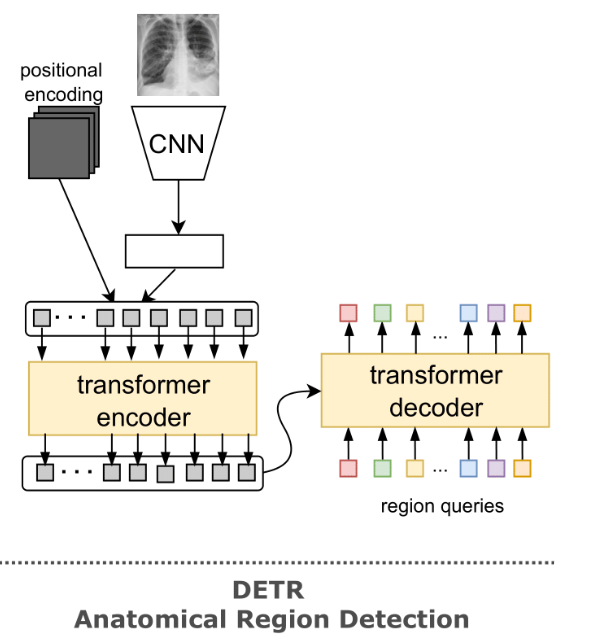
\includegraphics[width=1\linewidth]{assets/DETR.png}
    \caption{DETR Model}
    \label{fig:enter-label}
\end{figure}

We selected DETR for its end-to-end object detection and segmentation capabilities. Using transfer learning, we adapted DETR to the MIMIC-CXR dataset, enabling accurate segmentation of lung regions. The features extracted during segmentation were then used for downstream disease classification tasks.\\

\begin{figure}[H]
    \centering
    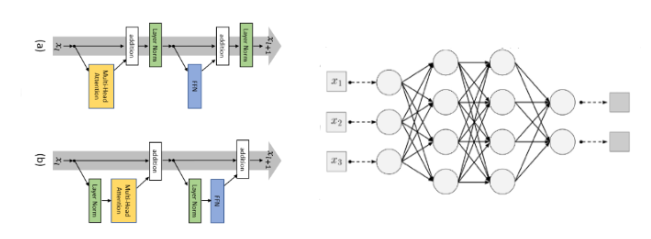
\includegraphics[width=1\linewidth]{assets/Disease_Classification.png}
    \caption{Disease Classification Model}
    \label{fig:enter-label}
\end{figure}

The disease classification model uses a layer transformer architecture\cite{2002.04745}, which calculates the attention of each feature to each other by comparing each feature to itself. Lastly feeding the features after attention balance to the linear layer to classify the disease.

\section{Dataset}
We are using the ImaGenome dataset, which contains 237,827 CXR Images annotated with the locations of 12 distinct anatomical regions and labels for 9 diseases. The dataset was divided into three subsets: Train(70\%), Validation(10\%), Test(20\%).\\


\begin{figure}[H]
    \centering
    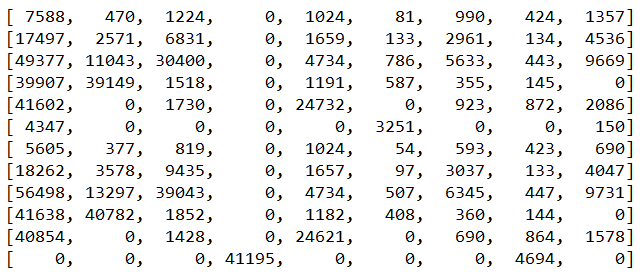
\includegraphics[width=1\linewidth]{assets/dataset.png}
    \caption{Occurrence of diseases in anatomical regions (i) across different conditions (j).}
    \label{fig:enter-label}
\end{figure}

Through data analysis, we found that in certain regions, the number of cases for some diseases is zero, and there is a significant disparity. Due to these reasons, the features of certain diseases cannot be learned effectively. Incorporating class weights for different diseases into the loss function \cite{1708.02002} can lead to performance improvements. However, in most cases, the improvement is marginal.\\

Given the pronounced imbalance in the dataset, relying solely on accuracy to evaluate model performance is inadequate, as it skews results and underestimates the model’s ability to detect minority classes. For such imbalanced datasets, ROC curves (Receiver Operating Characteristic) and AUC (Area Under the Curve) provide a more robust and suitable measure of performance.

\section{Results}
Our framework delivers standout performance across two pivotal tasks: anatomical region detection and disease classification. \\

In region detection, our DETR model delivers remarkable precision across 12 clinically significant anatomical regions, laying a vital foundation for subsequent disease classification tasks - capitalize on the accurate localization provided by our Transformer-based framework, with features extracted by DETR serving as the critical input to the downstream classification model, thereby enhancing its effectiveness.

\begin{figure}[H]
    \centering
    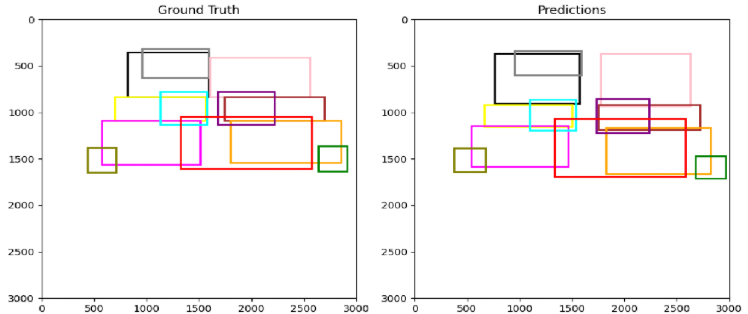
\includegraphics[width=1\linewidth]{assets/detr_performance.png}
    \caption{DETR Model Example}
    \label{fig:enter-label}
\end{figure}

For disease classification, we assessed our model’s performance using ROC curves and AUC metrics, achieving an average AUC of 83.7\% across a range of pathological conditions. This outcome underscores the model’s robust capability to distinguish diverse diseases with exceptional discriminative power.

\begin{figure}[H]
    \centering
    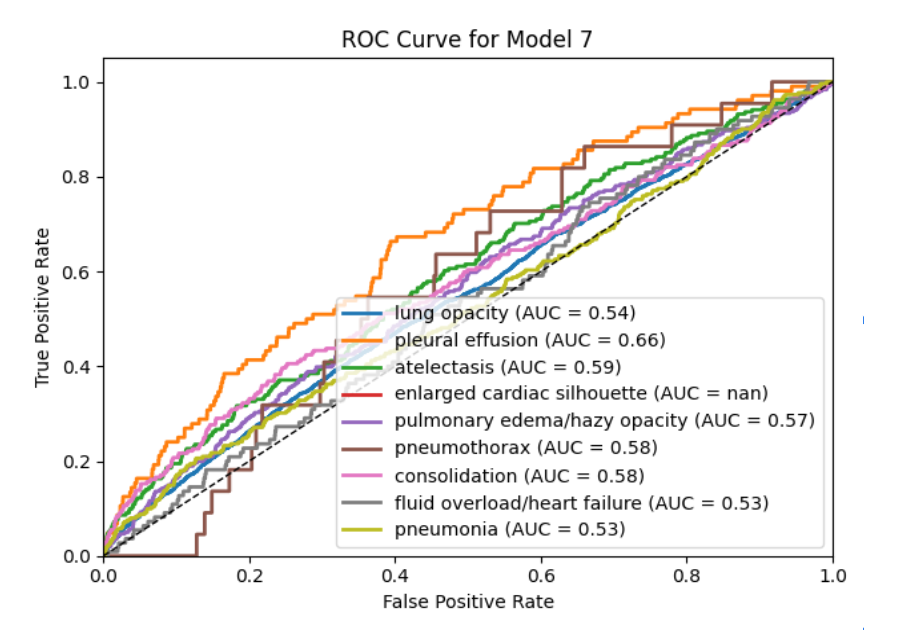
\includegraphics[width=1\linewidth]{assets/Region_7.png}
    \caption{DenseNet ROC Curve (Region 7)}
    \label{fig:enter-label}
\end{figure}

\begin{figure}[H]
    \centering
    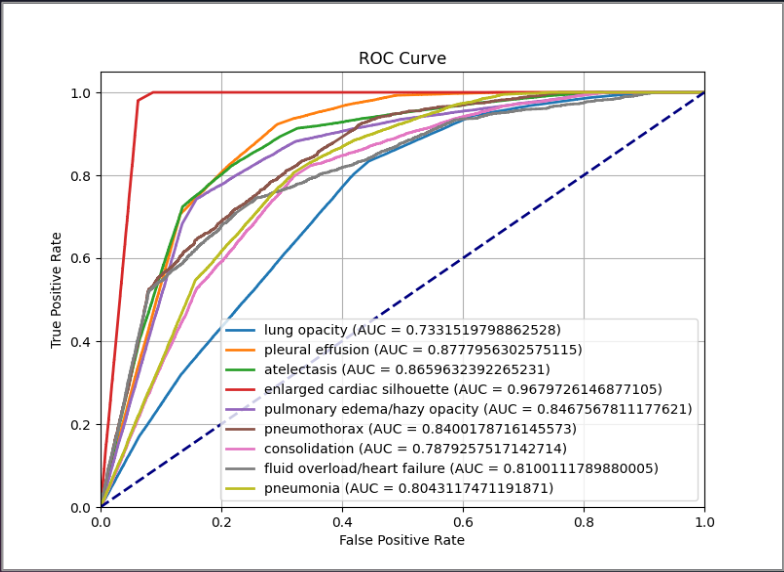
\includegraphics[width=1\linewidth]{assets/detr_roc.png}
    \caption{Our Model}
    \label{fig:enter-label}
\end{figure}

Compared to baseline approaches, our model achieves a substantially higher ROC score, reflecting its superior performance in disease classification tasks. .

\section{Conclusions}
In this study, we introduced a Detection Transformer (DETR)-based framework that unifies anatomical region detection and disease classification for comprehensive chest X-ray (CXR) analysis. By leveraging localized Transformer representations, our approach achieves robust performance, with a mean average precision (mAP) of 85\% for detecting clinically significant anatomical regions and an average ROC-AUC of 83.7\% across multiple pathological conditions. These results highlight the power of integrating precise localization with global contextual understanding, offering a computationally efficient alternative to conventional end-to-end models. Our framework not only advances the state of the art in medical image analysis but also provides a clinically actionable tool that aligns with the nuanced demands of radiological interpretation.

\section{Future Work}
While our framework achieves robust performance, several avenues remain for enhancement. One key direction involves integrating text extracted from Digital Imaging and Communications in Medicine (DICOM) metadata, which often contains patient history, imaging parameters, and preliminary radiologist notes. By developing a pipeline to parse and preprocess DICOM text—using natural language processing (NLP) techniques such as named entity recognition and context-aware embeddings—we could enrich the model’s input features. Combining these textual insights with our localized anatomical and pathological representations may enable more accurate and contextually informed disease detection. Furthermore, this approach could facilitate automated radiology report generation by aligning detected abnormalities with standardized clinical terminology, improving both precision and interpretability. Additional efforts will focus on addressing dataset imbalance through synthetic data generation and extending the framework to multi-modal imaging, such as incorporating computed tomography (CT) scans, to broaden its diagnostic scope.

\section*{Acknowledgements}
We would like to acknowledge the Department of Computing and Software at McMaster University (CAS) for providing the computational infrastructure necessary for model training.\\\\
We thank Dr. Mehdi Moradi for his supervision of the project, as well as for providing his insightful advice, guidance, and directions the research.\\\\
Lastly, Dr. Spencer Smith for providing the opportunity to this project\\\\

\begin{thebibliography}{99}
    \bibitem{irvin2019chexpert}
    Irvin, J., Rajpurkar, P., Ko, M., Yu, Y., Ciurea-Ilcus, S., et al., \textit{Chexpert: A large chest radiograph dataset with uncertainty labels and expert comparison}, 2019, arXiv preprint arXiv:1901.07031.

    \bibitem{johnson2019mimiccxr}
    Johnson, A.E., Pollard, T.J., Berkowitz, S.J., et al., \textit{Mimic-cxr, a de-identified publicly available database of chest radiographs with free-text reports}, 2019, Scientific Data, 1--8.

    \bibitem{rajpurkar2017chexnet}
    Rajpurkar, P., Irvin, J., Zhu, K., et al., \textit{Chexnet: Radiologist-level pneumonia detection on chest x-rays with deep learning}, 2017, arXiv preprint arXiv:1711.05225.

    \bibitem{wu2020comparison}
    Wu, J.T., Wong, K.C.L., Gur, Y., et al., \textit{Comparison of Chest Radiograph Interpretations by Artificial Intelligence Algorithm vs Radiology Residents}, 2020, JAMA Network Open, 3(10), e2022779.

    \bibitem{agu2021anaxnet}
    Agu, N.N., Wu, J.T., Chao, H., Lourentzou, I., Sharma, A., Moradi, M., Yan, P., Hendler, J., \textit{Anaxnet: Anatomy aware multi-label finding classification in chest x-ray}, 2021, Medical Image Computing and Computer Assisted Intervention -- MICCAI 2021, Springer, 804--813.

    \bibitem{carion2020end}
    Carion, N., Massa, F., Synnaeve, G., Usunier, N., Kirillov, A., Zagoruyko, S., \textit{End-to-end object detection with transformers}, 2020, European Conference on Computer Vision (ECCV), Springer, 213--229.

    \bibitem{1608.06993}
    Huang, G., Liu, Z., van der Maaten, L., Weinberger, K.Q., \textit{Densely Connected Convolutional Networks}, 2016, arXiv:1608.06993.

    \bibitem{1812.08434}
    Zhou, J., Cui, G., Hu, S., Zhang, Z., Yang, C., Liu, Z., Wang, L., Li, C., Sun, M., \textit{Graph Neural Networks: A Review of Methods and Applications}, 2018, arXiv:1812.08434.

    \bibitem{2010.11929}
    Dosovitskiy, A., Beyer, L., Kolesnikov, A., Weissenborn, D., Zhai, X., Unterthiner, T., Dehghani, M., Minderer, M., Heigold, G., Gelly, S., Uszkoreit, J., Houlsby, N., \textit{An Image is Worth 16x16 Words: Transformers for Image Recognition at Scale}, 2020, arXiv:2010.11929.

    \bibitem{2103.14899}
    Chen, C.F., Fan, Q., Panda, R., \textit{CrossViT: Cross-Attention Multi-Scale Vision Transformer for Image Classification}, 2021, arXiv:2103.14899.

    \bibitem{2002.04745}
    Xiong, R., Yang, Y., He, D., Zheng, K., Zheng, S., Xing, C., Zhang, H., Lan, Y., Wang, L., Liu, T.Y., \textit{On Layer Normalization in the Transformer Architecture}, 2020, ICML 2020.

    \bibitem{1708.02002}
    Lin, T.Y., Goyal, P., Girshick, R., He, K., Dollár, P., \textit{Focal Loss for Dense Object Detection}, 2017, arXiv:1708.02002.
\end{thebibliography}

\clearpage
\onecolumn
\begin{landscape}
\begin{figure}[htbp]
    \centering
    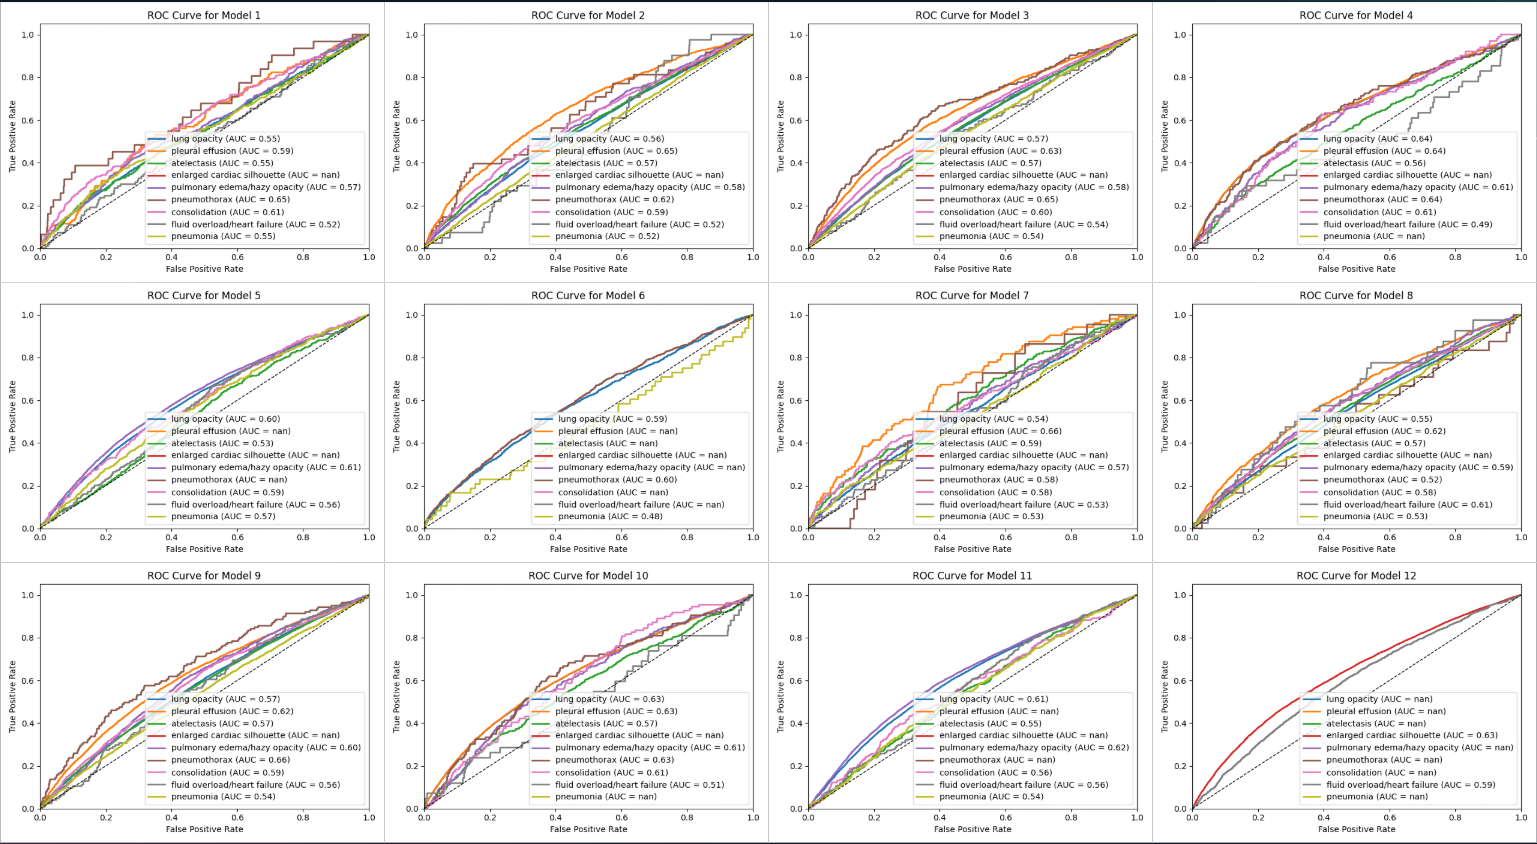
\includegraphics[width=1.35\textwidth]{assets/all_regions.png}
    \caption{DenseNet (All regions) - Including all 12 regions of the ROC curve.}
    \label{fig:enter-label}
\end{figure}
\end{landscape}
\end{document}